\documentclass[aspectratio=169]{beamer}
\usetheme{Madrid}
\usecolortheme{default}

%% USEPACKAGES %%
\usepackage{subcaption}
\usepackage{csquotes}
\usepackage{datetime}
\usepackage[british]{babel}
\usepackage[backend=biber]{biblatex}
\addbibresource{references.bib}

\usepackage{nameref}
\makeatletter
\newcommand*{\currentname}{\@currentlabelname}
\makeatother

\usepackage{subcaption}
\usepackage{listings}
\usepackage{lipsum}
\definecolor{codegreen}{rgb}{0,0.6,0}
\definecolor{codegray}{rgb}{0.5,0.5,0.5}
\definecolor{codepurple}{rgb}{0.58,0,0.82}
\definecolor{backcolour}{rgb}{0.95,0.95,0.92}

\lstdefinestyle{mypython}{
    backgroundcolor=\color{backcolour},
    commentstyle=\color{codegreen},
    keywordstyle=\color{magenta},
    numberstyle=\tiny\color{codegray},
    stringstyle=\color{codepurple},
    basicstyle=\ttfamily\footnotesize,
    breakatwhitespace=false,
    breaklines=true,
    captionpos=b,
    keepspaces=true,
    numbers=left,
    numbersep=5pt,
    showspaces=false,
    showstringspaces=false,
    showtabs=false,
    tabsize=2,
}
\lstset{language=Python,
  style=mypython}

%% BEAMER CONFIG %%
\definecolor{uosblue}{RGB}{1,91,130}
\definecolor{gradient1}{RGB}{2, 110, 156}
\definecolor{gradient2}{RGB}{0, 72, 104}
\setbeamercolor{author in head/foot}{fg=white, bg=gradient1}
\setbeamercolor{title in head/foot}{fg=white, bg=uosblue}
\setbeamercolor{date in head/foot}{fg=white, bg=gradient2}
\setbeamercolor{section in head/foot}{fg=white, bg=uosblue}
\setbeamercolor{titlelike}{fg=white,bg=uosblue}

\setbeamertemplate{item}{bg=uosblue}
\setbeamertemplate{enumerate items}[default]
\setbeamertemplate{itemize items}[default]
\setbeamerfont{title}{series=\bfseries}
\setbeamercolor*{palette primary}{fg=white,bg=uosblue}
\setbeamercolor*{palette secondary}{fg=white, bg=uosblue}
\beamertemplatenavigationsymbolsempty
\setbeamertemplate{caption}[numbered]
\setbeamertemplate{date}{}%


\AtBeginSection[]
{
    \begin{frame}
        \frametitle{}
        \centering
        \huge{\currentname}
    \end{frame}
}

%% DOCUMENT INFO %%
\title[From SNNs to Silicon]
{From SNNs to Silicon:\\\emph{Compiling FPGA Bitstreams from Spiking Neural Networks}}


\author[Michail Rontionov]{
  \textbf{Michail Rontionov}$^{1\dagger}$,
  Jens E. Pedersen$^{2\ddagger}$,
  Charlotte Frenkel$^{3}$,\\
  Francisco Ayala Le Brun$^{3}$,
  Nassim Beladel$^{4}$\\
  \vspace{1em}
  Emails: $^{\dagger}$ \texttt{m.rontionov@soton.ac.uk}, $^{\ddagger}$ \texttt{jegpe@dtu.dk}
}

% \newdateformat{monthyeardate}{%
%   \monthname[\THEMONTH] \THEYEAR}
%
% \date{\monthyeardate\today}

\titlegraphic{%
  \centering
  \begin{columns}[c]
    \begin{column}{0.45\textwidth}
      \centering
      $\vcenter{\hbox{
\includegraphics[height=1cm]{img/uos.png}}}^{1}$\hspace{0.5em}%
      $\vcenter{\hbox{
\includegraphics[height=1cm]{img/mindscdt.png}}}^{1}$\hspace{0.5em}%
      $\vcenter{\hbox{
\includegraphics[height=1cm]{img/ukri.png}}}^{1}$
    \end{column}
    \hfill
    \begin{column}{0.45\textwidth}
      \centering
      $\vcenter{\hbox{
\includegraphics[height=1cm]{img/dtu.jpg}}}^{2}$
      $\vcenter{\hbox{
\includegraphics[height=0.8cm]{img/delft.png}}}^{3}$\hspace{1em}%
      $\vcenter{\hbox{
\includegraphics[height=0.4cm]{img/eth.png}}}^{4}$\hspace{1em}%

    \end{column}
  \end{columns}%
}

\begin{document}
\frame{\titlepage}

\begin{frame}{Why this tutorial?}
  \begin{columns}
    \begin{column}{.5\textwidth}
      \begin{itemize}
      \item Neuromorphic computing addresses
      \end{itemize}

    \end{column}

    \begin{column}{.5\textwidth}

    \end{column}
  \end{columns}
\end{frame}

\begin{frame}{What is Neuromorphic Computing?}
\begin{columns}
  \begin{column}{.6\textwidth}
    \begin{itemize}[<+->]
    \item \textbf{Neuromorphic Computing}: Exploring parallels between biological neurons and neural computation.
    \item \textbf{Spiking Neural Networks} (SNNs): Neural networks with time domain and more \emph{realistic neuron models}.
    \item \textbf{Differences} compared to Artificial NNs:
      \begin{itemize}
      \item \emph{Sparsity}: Typical ANNs such as AlexNet or VGG models exhibit 60-70\% activiaton sparsity. SNNs can get up to 99\%.
      \item \emph{Localised Learning}: Time domain enables novel bio-inspired, robust learning algorithms.
      \item \emph{Energy Efficiency}: Event-driven, sparse computation translates to orders-of-magnitude lower power on neuromorphic hardware \cite{snn}.
      \end{itemize}
    \end{itemize}
  \end{column}

  \begin{column}{.4\textwidth}
    \begin{figure}[ht]
      \centering
      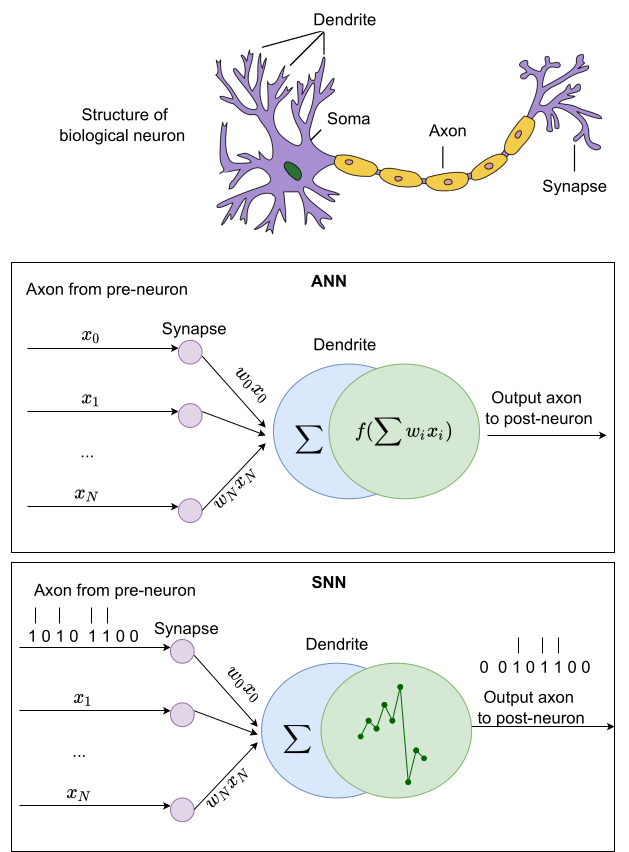
\includegraphics[width=4.5cm]{img/x7.png}
      \caption*{\tiny Biological neuron vs Artificial Neural Network (ANN) vs Spiking Neural Network (SNN) (as in \cite{snn})}
    \end{figure}

  \end{column}
\end{columns}
\end{frame}

\begin{frame}[plain]
  \Huge
  \centering
  Temporary slide
\end{frame}

% \begin{frame}{NIR-Centric Hardware Design}
%   \begin{columns}
%     \begin{column}{.5\textwidth}
%       \begin{figure}[htbp]
%         \centering
%         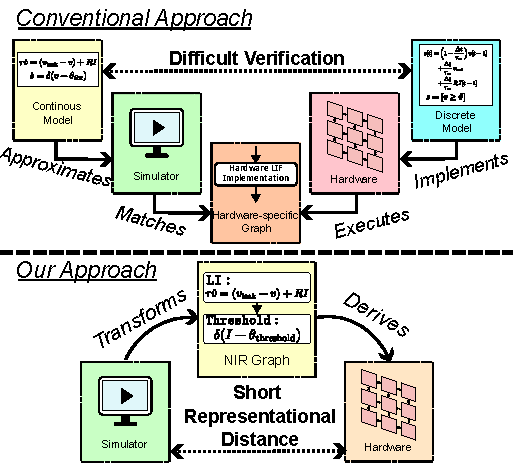
\includegraphics[width=0.8\textwidth]{img/flow2.pdf}
%         \caption{\label{lol1} Conventional hardware design vs our proposal.}
%       \end{figure}
%     \end{column}

%     \begin{column}{.5\textwidth}
%       \begin{figure}[htbp]
%         \centering
%         
\includegraphics[width=1.0\textwidth]{/home/mrontio/uni/phd/documents/publications/nir-fpga-publication/img/architecture.pdf}
%         \label{lol2}
%         \caption{ An example generation of our toolchain from an SNN with the CuBa-LIF neuron model.}

%       \end{figure}
%     \end{column}
%   \end{columns}


% \end{frame}


\end{document}
%%% Local Variables:
%%% mode: latex
%%% TeX-master: t
%%% End:
